\chapter*{Dodatak: Prikaz aktivnosti grupe}
		\addcontentsline{toc}{chapter}{Dodatak: Prikaz aktivnosti grupe}
		
		\section*{Dnevnik sastajanja}
		
		%&\textbf{\textit{Kontinuirano osvježavanje}}\\
		%\textit{U ovom dijelu potrebno je redovito osvježavati dnevnik sastajanja prema predlošku.}
		
		\begin{packed_enum}
			\item  sastanak
			\item[] \begin{packed_item}
				\item Datum: 19. listopada 2023.
				\item Prisustvovali: L. Miličević, M. Papak, F. Aleksić, S. Đelekovčan, D. Sviličić, E. Pužar
				\item Teme sastanka:
				\begin{packed_item}
					\item  sastanak s asistenticom i demonstratorom
					\item  uvod u temu projekta
				\end{packed_item}
			\end{packed_item}

			\item  sastanak
			\item[] \begin{packed_item}
				\item Datum: 22. listopada 2023.
				\item Prisustvovali: L. Miličević, M. Papak, F. Aleksić, D. Huljev, S. Đelekovčan, D. Sviličić, E. Pužar
				\item Teme sastanka:
				\begin{packed_item}
					\item  analiza teme projekta
					\item  korištenje git-a i github-a
					\item  konačan odabir alata i tehnologija
					\item  uvod u naš github repozitorij
				\end{packed_item}
			\end{packed_item}
			
			\item  sastanak
			\item[] \begin{packed_item}
				\item Datum: 30. listopada 2023.
				\item Prisustvovali: L. Miličević, D. Huljev, S. Đelekovčan, D. Sviličić, E. Pužar
				\item Teme sastanka:
				\begin{packed_item}
					\item  definiranje funkcionalnih zahtjeva
					\item  podjela opisa obrazaca uporabe, opisa zadatka i arhitekture sustava
				\end{packed_item}
			\end{packed_item}

			\item  sastanak
			\item[] \begin{packed_item}
				\item Datum: 2. studenoga 2023.
				\item Prisustvovali: L. Miličević, M. Papak, F. Aleksić, D. Huljev, S. Đelekovčan, D. Sviličić, E. Pužar
				\item Teme sastanka:
				\begin{packed_item}
					\item  analiza do sada napravljenih funkcionalih zahtjeva
					\item  diskusija o modeliranju baze podataka
				\end{packed_item}
			\end{packed_item}

			\item  sastanak
			\item[] \begin{packed_item}
				\item Datum: 9. studenoga 2023.
				\item Prisustvovali: L. Miličević, M. Papak, F. Aleksić, D. Huljev, S. Đelekovčan, D. Sviličić, E. Pužar
				\item Teme sastanka:
				\begin{packed_item}
					\item  sastanak i diskusija s asistentom
				\end{packed_item}
			\end{packed_item}

			\item  sastanak
			\item[] \begin{packed_item}
				\item Datum: 12. studenoga 2023.
				\item Prisustvovali: L. Miličević, M. Papak, F. Aleksić, D. Huljev, S. Đelekovčan, D. Sviličić, E. Pužar
				\item Teme sastanka:
				\begin{packed_item}
					\item  zajednička implementacija frontend dijela generičkih funkcionalnosti
				\end{packed_item}
			\end{packed_item}

			\item  sastanak
			\item[] \begin{packed_item}
				\item Datum: 18. prosinca 2023.
				\item Prisustvovali: L. Miličević, M. Papak, F. Aleksić, D. Huljev, S. Đelekovčan, D. Sviličić, E. Pužar
				\item Teme sastanka:
				\begin{packed_item}
					\item plan nastavka rada na projektu
					\item podjela poslova
				\end{packed_item}
			\end{packed_item}

			\item  sastanak
			\item[] \begin{packed_item}
				\item Datum: 3. siječnja 2023.
				\item Prisustvovali: L. Miličević, M. Papak, F. Aleksić, D. Huljev, S. Đelekovčan, D. Sviličić, E. Pužar
				\item Teme sastanka:
				\begin{packed_item}
					\item detaljnija podjela dužnosti
				\end{packed_item}
			\end{packed_item}

			\item  sastanak
			\item[] \begin{packed_item}
				\item Datum: 9. siječnja 2023.
				\item Prisustvovali: L. Miličević, M. Papak, F. Aleksić, D. Huljev, S. Đelekovčan, D. Sviličić, E. Pužar
				\item Teme sastanka:
				\begin{packed_item}
					\item praćenje napretka implementacije funkcionalnosti
					\item diskusija o problemima i rješenjima
					\item plan nastavka rada
				\end{packed_item}
			\end{packed_item}

			\item  sastanak
			\item[] \begin{packed_item}
				\item Datum: 16. siječnja 2023.
				\item Prisustvovali: L. Miličević, M. Papak, F. Aleksić, D. Huljev, S. Đelekovčan, D. Sviličić, E. Pužar
				\item Teme sastanka:
				\begin{packed_item}
					\item plan o završetku zadatka
					\item riješavanje problema s implementacijom
				\end{packed_item}
			\end{packed_item}
			
			%
			
		\end{packed_enum}
		
		\eject
		\section*{Tablica aktivnosti}
		
			%\textbf{\textit{Kontinuirano osvježavanje}}\\
			
			%\textit{Napomena: Doprinose u aktivnostima treba navesti u satima po članovima grupe po aktivnosti.}

			\begin{longtblr}[
					label=none,
				]{
					vlines,hlines,
					width = \textwidth,
					colspec={X[7, l]X[1, c]X[1, c]X[1, c]X[1, c]X[1, c]X[1, c]X[1, c]}, 
					vline{1} = {1}{text=\clap{}},
					hline{1} = {1}{text=\clap{}},
					rowhead = 1,
				} 
			
				\SetCell[c=1]{c}{} & \SetCell[c=1]{c}{\rotatebox{90}{\textbf{Luka Miličević}}} & \SetCell[c=1]{c}{\rotatebox{90}{\textbf{Duje Huljev}}} &	\SetCell[c=1]{c}{\rotatebox{90}{\textbf{Filip Aleksić}}} & \SetCell[c=1]{c}{\rotatebox{90}{\textbf{Mate Papak}}} &	\SetCell[c=1]{c}{\rotatebox{90}{\textbf{Stjepan Đelekovčan}}} & \SetCell[c=1]{c}{\rotatebox{90}{\textbf{Domagoj Sviličić}}} &	\SetCell[c=1]{c}{\rotatebox{90}{\textbf{Erik Pužar}}} \\  
				Upravljanje projektom 		& 3 &  &  &  &  &  & \\ 
				Opis projektnog zadatka 	& 3 &  &  &  &  &  & \\ 
				
				Funkcionalni zahtjevi       &  & 4 & 3 & 2 &  & 3 & 3 \\ 
				Opis pojedinih obrazaca 	&  & 3 & 3 & 3 &  & 2 & 3 \\ 
				Dijagram obrazaca 			&  & 3 & 2 & 2 &  & 1 & 2 \\ 
				Sekvencijski dijagrami 		&  & 1 &  &  &  & 4 & 4 \\ 
				Opis ostalih zahtjeva 		& 0.5 &  &  &  &  &  &  \\ 

				Arhitektura i dizajn sustava	& 2 &  &  &  &  &  &  \\ 
				Baza podataka					&  &  &  &  & 9 &  &   \\ 
				Dijagram razreda 				& 7 &  &  &  &  &  &   \\ 
				Dijagram stanja					&  & 3 &  &  &  &  &  \\ 
				Dijagram aktivnosti 			&  &  &  &  &  & 6 & \\ 
				Dijagram komponenti				&  &  &  &  &  & 9 &  \\ 
				Korištene tehnologije i alati 		&  &  &  &  &  & 4 & \\ 
				Ispitivanje programskog rješenja 	& 3 &  & 14 & 9 &  &  &  \\
				Dijagram razmještaja			&  &  &  &  &  & 6 &  \\ 
				Upute za puštanje u pogon 		&  &  &  &  &  &  &  \\  
				Dnevnik sastajanja 			& 1 &  &  &  &  &  &  \\ 
				Zaključak i budući rad 		&  &  &  &  &  & 3 & \\  
				Popis literature 			& 1 &  &  &  &  &  &  \\  
				&  &  &  &  &  &  &  \\ \hline 
				Inciijalno postavljanje frontenda aplikacije 			& 7 &  &  &  &  &  &  \\  
				Inicijalno postavljanje backenda aplikacije 			& 1 &  &  &  & 6 &  &  \\  
				Generičke funkcionalnosti - Login i Registracija 		& 5 & 1 & 1 & 1 & 11 & 1 & 2 \\  
				Puštanje aplikacije u pogon 							& 5 &  &  &  &  &  &  \\  
				Infrastruktura i uređenje frontenda aplikacije 					& 15 & 2 &  &  &  &  & 1 \\
				Infrastruktura i uređenje backenda aplikacije 					& 2 &  &  &  & 6 &  & 1 \\
				Izrada infrastrukuture za rad sa slikama 				&  & 1 &  &  & 4 &  &  \\
				Stranica za korisnički račun 							& 1 & 1 &  &  & 15 &  & 2 \\
				Stranica za javni profil 							&  & 1 &  & 11 &  &  &  \\
				Stranice za pretplatu i administraciju 				& 4 &  &  &  & 3 &  & 8 \\
				Stranice za izradu i uređenje događaja 				& 4 & 12 &  & 12 & 6 &  & 2 \\
				Kartica za detalje o događaju 						&  &  & 8 &  &  &  &  \\
				Kartica za pregled događaja - sortiranje i filtriranje				& 2 &  & 9 &  &  &  &  \\
			\end{longtblr}
					
					
		\eject
		\section*{Dijagrami pregleda promjena}

		Komentar na pregled izmjena: prikaz nije u potpunosti točan i prikazuje manje promjena za dio tima koji nije sam merge-ao svoje grane u develop ili devdoc grane.
		
		\begin{figure}[htbp]
			\centering
			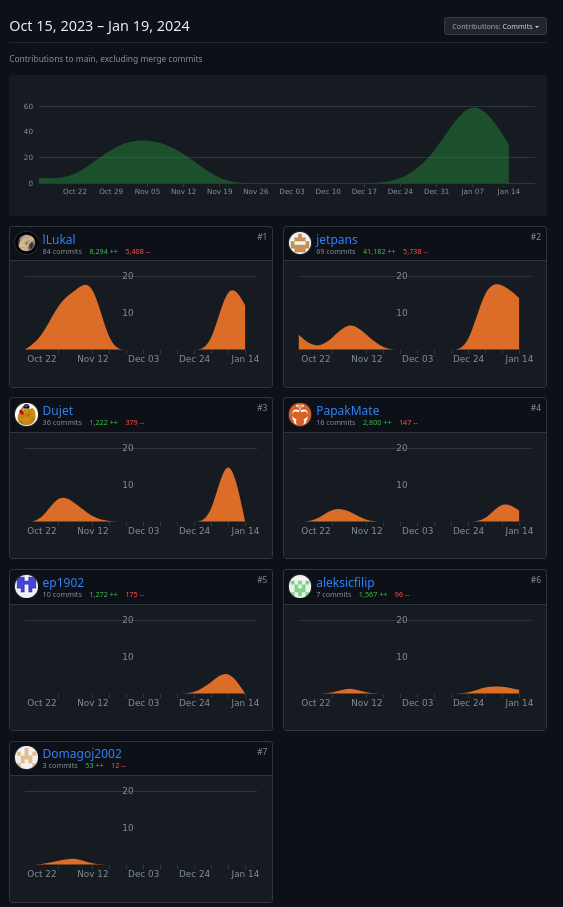
\includegraphics[width=0.9\textwidth]{slike/pregled_promjena.png}
			\caption{Dijagram pregleda promjena}
		\label{fig:my_image}
		\end{figure}
		\eject
	